\chapter{Preliminary Work}
	
	\section{High-Speed Serial Link Modelling}
		
		In order to understand the effects of inserting non-uniformity to the
		SpiNNaker Interconnect caused by the high speed links.
		
		\subsection{Objectives}
			Try and find out what is going on.
		
		\subsection{Results}
			Found a significant increase in average latency. Maybe this could be
			overcome by making more use of that added processing time by jumping on
			further ahead? Further simulation needs to be done anyhow...
	
	\section{SpiNNaker PCI-Express Interface}
		
		One way of getting data from one part of the machine to the other would be
		not to just dump it through another link but to pull it straight out into a
		conventional computer via PCI-Express and then maybe re-route it with
		fancier software or via the web.
		
		\subsection{PCI-Express}
			
			What is PCI-Express? How does it work? Where is it found?
		
		\subsection{High Speed Serial on FPGA}
			
			What is an FPGA? We have one on the boards. FPGAs contain hard-wired
			blocks which do special purpose things, one such job is to do PCI-Express.
	
	\section{Wiring-Up Large SpiNNaker Machines}
		
		% A practical constraint on any interconnect is that it should be possible to
		% wire it up. In particular constraints exist on both on wire length and the
		% practical difficulty of connecting up the wires into the correct places.
		% Computers usually placed in racks. Tool can be used to study wiring
		% constraints of new links.
		
		One of the practical constraints on the topologies which super-computers are
		able to exploit is the use of wires to connect parts of the system together.
		Chief amongst these concerns are the following:
		
		\begin{description}
			
			\item[Wire Cost] The choice of cabling used has a direct impact on the
			financial cost of the wiring. Higher quality materials or increased
			numbers of wires can substantially drive up the cost of the cable and
			connectors required.
			
			\item[Wire Length] Long wires have higher capacitances than short ones
			which limits the rate at which data can be transmitted.
			
			\item[Wiring Complexity] Ultimately the system will need to be assembled
			(presumably) by hand and so keeping wiring patterns simple is important to
			reduce the number of wiring mistakes.
			
		\end{description}
		
		The SpiNNaker interconnect topology was studied to confirm the existence of
		a practical wiring scheme for the machine which satisfies all of the above
		properties. The principles of the machine's construction suggested by
		Davidson \cite{davidsonWiring} and Furber \cite{furber13email} were used as
		the basis for a tool used to model and experiment with possible
		configurations. This section explains the mapping developed and how it
		meets the above requirements. Finally, the section concludes with a
		description of the tool and the future work which remains.
		
		\subsection{SpiNNaker Boards}
			
			% SpiNNaker has three dimensions of wiring connected in a torus. This has
			% long wires. A torus intuitively has long wires along the way which causes
			% a bit of a headache. You can slice it to make it rectangular, you can fold
			% it to make the wires short (must fold 4x2) and divvy up into cabinets..
			
			% TODO SpiNNaker topology back reference
			
			The SpiNNaker topology, as described in \S\ref{sec:todo}, consists of a
			regular 2D grid of 18-core chips arranged in a toroid with
			nearest-neighbour links travelling North, North-East and East. The
			complete system will host 57,600 chips which are split up into 1,200
			circuit boards of 48 chips each (Figure \ref{fig:spinn4labelled}). These
			boards are equipped with a number of high-speed links, six of which are
			used to connect them to their neighbours, the others are reserved for
			other I/O.
			
			\begin{figure}
				\center
				\begin{tikzpicture}[thick]
	
	\node[anchor=south west,inner sep=0] at (0,0) (image)
		{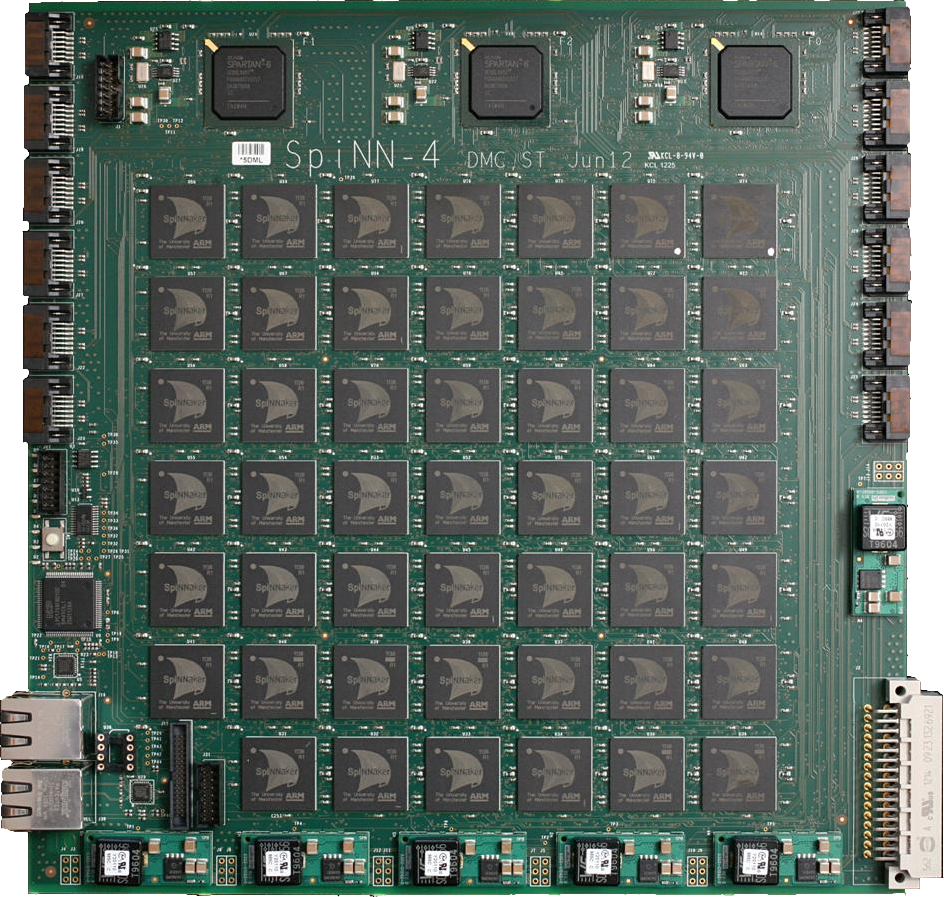
\includegraphics[width=0.5\textwidth]{figures/spinn4.png}};
	
	\begin{scope}[x={(image.south east)},y={(image.north west)}]
		%% Help with drawing
		%\draw[help lines,xstep=.1,ystep=.1] (0,0) grid (1,1);
		%\foreach \x in {0,1,...,9} { \node [anchor=north] at (\x/10,0) {0.\x}; }
		%\foreach \y in {0,1,...,9} { \node [anchor=east] at (0,\y/10) {0.\y}; }
		
		\draw [decorate,decoration={brace,raise=1ex,amplitude=1ex}]
		      (0.02,0.5) -- coordinate (left-label) (0.02,1.0);
		\node [left=1em of left-label,text width=3.5cm,align=center]
		      {High-Speed Links\\(Board-to-Board)};
		
		\draw [decorate,decoration={brace,raise=1ex,amplitude=1ex}]
		      (0.97,1.0) -- coordinate (right-label) (0.97,0.5);
		\node [right=1em of right-label,text width=3.5cm,align=center]
		      {High-Speed Links\\(Other I/O)};
		
		\draw [decorate,decoration={brace,raise=1ex,amplitude=1ex}]
		      (1.0,0.23) -- coordinate (power-label) (1.0,0.02);
		\node [right=1em of power-label] {Power Connector};
		
		\draw [decorate,decoration={brace,raise=1ex,amplitude=1ex}]
		      (0.0,0.08) -- coordinate (eth-label) (0.0,0.22);
		\node [left=1em of eth-label] {Ethernet};
	\end{scope}
	
\end{tikzpicture}

				\caption{48-chip SpiNNaker Circuit Board}
				\label{fig:spinn4labelled}
			\end{figure}
			
			The chips on each circuit board are logically laid out as shown in Figure
			\ref{fig:chipsOnBoard}. Touching edges represent a chip-to-chip connection
			and the outer connections are connected to chips on neighbouring boards.
			In order to reduce the number of wires required, the board-to-board
			connections are carried via six high-speed links (labelled in the figure)
			each carrying 8 chip-to-chip connections. The six directions correspond to
			the six high-speed link connectors on the board used for board-to-board
			links.
			
			By concentrating several connections onto one high-speed link the number
			of wires is cut from 128 to 4. This substantially reduces the cost of the
			cables and connectors involved, satisfying the `wire cost' concern.
		
		\subsection{Connecting Boards Together}
			
			\label{ref:connectingBoardsTogether}
			
			\begin{figure}
				\center
				\begin{tikzpicture}[thick,scale=0.8,inner sep=0]
	\begin{scope}[hexagonXYZ]
		\foreach \x/\y/\num in {%
		                                          0/4/45,   1/4/46,   2/4/47,   3/4/48, %
		                                -1/3/44,  0/3/25,   1/3/26,   2/3/27,   3/3/28, %
		                      -2/2/43,  -1/2/24,  0/2/11,   1/2/12,   2/2/13,   3/2/29, %
		            -3/1/42,  -2/1/23,  -1/1/10,  0/1/3,    1/1/4,    2/1/14,   3/1/30, %
		  -4/0/41,  -3/0/22,  -2/0/9,   -1/0/2,   0/0/1,    1/0/5,    2/0/15,   3/0/31, %
		  -4/-1/40, -3/-1/21, -2/-1/8,  -1/-1/7,  0/-1/6,   1/-1/16,  2/-1/32,          %
		  -4/-2/39, -3/-2/20, -2/-2/19, -1/-2/18, 0/-2/17,  1/-2/33,                    %
		  -4/-3/38, -3/-3/37, -2/-3/36, -1/-3/35, 0/-3/34,                              %
		}{
		  \node [draw,hexagon,minimum size=0.8cm,inner sep=0,font=\footnotesize]
		        at (\x,\y) (chip \num) {\num};
		}
	\end{scope}
	
	\newcommand{\spinnbrace}[5]{
		\draw [decorate,decoration={brace,amplitude=1ex,raise=1ex}]
		      (#1) -- coordinate (label) (#2);
		\node at (label) [shift={(#3:1.5em))}] [#5] {#4};
	}
	
	\spinnbrace{chip 45.side north}{chip 48.side north east}{90}{North}{};
	
	\spinnbrace{chip 41.side north}{chip 45.side west}{150}{West}{xshift=-0.8em};
	
	\spinnbrace{chip 38.side south west}{chip 41.side west}{-150}{South-West}{xshift=-2.1em};
	
	\spinnbrace{chip 34.side south west}{chip 38.side south}{-90}{South}{};
	
	\spinnbrace{chip 31.side east}{chip 34.side south}{-30}{East}{xshift=0.8em};
	
	\spinnbrace{chip 48.side east}{chip 31.side north east}{30}{North-East}{xshift=2.2em};
	
	
\end{tikzpicture}

				\caption{Logical arrangement of chips on a circuit board}
				\label{fig:chipsOnBoard}
			\end{figure}
			
			In order to construct a toroid, at least three boards  must be combined as
			shown in Figure \ref{fig:threeboard} (known as a threeboard).  Figure
			\ref{fig:threeboardSliced} shows how the threeboard arrangement can be
			turned into a sheet which in turn can be turned into a toroid by connecting
			the opposing sides.
			
			\begin{figure}
				\begin{subfigure}[b]{0.45\textwidth}
					\center
					\begin{tikzpicture}[thick,scale=0.3,inner sep=0]
	\begin{scope}[hexagonXYZ]
		\foreach \xoff/\yoff/\colour in {%
			0/0/red,%
			4/8/green,%
			8/4/blue%
		}{
			\foreach \x/\y/\num in {%
			                                          0/4/45,   1/4/46,   2/4/47,   3/4/48, %
			                                -1/3/44,  0/3/25,   1/3/26,   2/3/27,   3/3/28, %
			                      -2/2/43,  -1/2/24,  0/2/11,   1/2/12,   2/2/13,   3/2/29, %
			            -3/1/42,  -2/1/23,  -1/1/10,  0/1/3,    1/1/4,    2/1/14,   3/1/30, %
			  -4/0/41,  -3/0/22,  -2/0/9,   -1/0/2,   0/0/1,    1/0/5,    2/0/15,   3/0/31, %
			  -4/-1/40, -3/-1/21, -2/-1/8,  -1/-1/7,  0/-1/6,   1/-1/16,  2/-1/32,          %
			  -4/-2/39, -3/-2/20, -2/-2/19, -1/-2/18, 0/-2/17,  1/-2/33,                    %
			  -4/-3/38, -3/-3/37, -2/-3/36, -1/-3/35, 0/-3/34,                              %
			}{
			  \node [draw,hexagon,minimum size=0.3cm,inner sep=0,font=\footnotesize,\colour]
			        at (\x+\xoff,\y+\yoff) (chip \num) {};
			}
		}
	\end{scope}
	
\end{tikzpicture}

					\caption{Threeboard}
					\label{fig:threeboard}
				\end{subfigure}
				\begin{subfigure}[b]{0.45\textwidth}
					\center
					\begin{tikzpicture}[thick,scale=0.3,inner sep=0]
	\begin{scope}[hexagonXYZ]
		\foreach \xoff/\yoff/\colour in {%
			0/0/red,%
			4/8/green,%
			8/4/blue%
		}{
			\foreach \x/\y/\num in {%
			                                          0/4/45,   1/4/46,   2/4/47,   3/4/48, %
			                                -1/3/44,  0/3/25,   1/3/26,   2/3/27,   3/3/28, %
			                      -2/2/43,  -1/2/24,  0/2/11,   1/2/12,   2/2/13,   3/2/29, %
			            -3/1/42,  -2/1/23,  -1/1/10,  0/1/3,    1/1/4,    2/1/14,   3/1/30, %
			  -4/0/41,  -3/0/22,  -2/0/9,   -1/0/2,   0/0/1,    1/0/5,    2/0/15,   3/0/31, %
			  -4/-1/40, -3/-1/21, -2/-1/8,  -1/-1/7,  0/-1/6,   1/-1/16,  2/-1/32,          %
			  -4/-2/39, -3/-2/20, -2/-2/19, -1/-2/18, 0/-2/17,  1/-2/33,                    %
			  -4/-3/38, -3/-3/37, -2/-3/36, -1/-3/35, 0/-3/34,                              %
			}{
				\pgfmathtruncatemacro{\xx}{\x+\xoff}
				\pgfmathtruncatemacro{\yy}{\y+\yoff}
				\ifthenelse{\xx < 0}{
					\pgfmathtruncatemacro{\xx}{\xx+12}
				}{}
				\ifthenelse{\yy > 8}{
					\pgfmathtruncatemacro{\yy}{\yy-12}
				}{}
				\node [draw,hexagon,minimum size=0.3cm,inner sep=0,font=\footnotesize,\colour]
				      at (\xx,\yy) (chip \num) {};
			}
		}
	\end{scope}
	
\end{tikzpicture}

					\caption{Sliced Into A Sheet}
					\label{fig:threeboardSliced}
				\end{subfigure}
				
				\caption[A `threeboard']{A `threeboard', the minimal configuration of boards yielding a
				toroid}
			\end{figure}
			
			Arbitrarily large systems can be created by repeating the threeboard
			pattern as shown in Figure \ref{fig:boardsLogical}. In the figure,
			touching boards are connected and the lines represent wires which complete
			the toroid by connecting opposing edges. It is clear that while the
			majority of wires are very short (they connect two boards which are
			side-by-side), some wires cross the entire system's length.
			
			\begin{figure}
				\center
				\input{|"python figures/boardsLogical.py"}
				\caption[Logical arrangement of boards in a $4\times4$ threeboard
				SpiNNaker system.]{Logical arrangement of boards in a $4\times4$
				threeboard SpiNNaker system. Touching boards are connected. Coloured
				lines represent long connections travelling {\color{red}North/South},
				{\color{green}North-East/South-West} and {\color{blue}East/West}}
				\label{fig:boardsLogical}
			\end{figure}
			
			To remove long wires from a toroid network, the network can be folded. An
			example of this process is shown for a simple ring-network (a
			1-dimensional toroid) in Figure \ref{fig:folding}.
			
			\begin{figure}
				\begin{subfigure}[b]{\textwidth}
					\center
					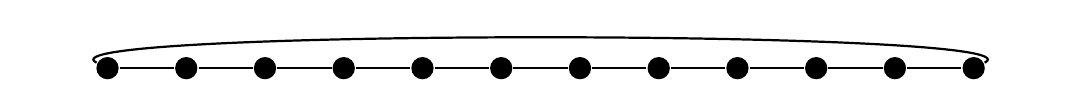
\begin{tikzpicture}[thick,inner sep=0.1cm]
	\node [fill,circle] (node 153942796) at (0.000000,0.000000) {};
	\node [fill,circle] (node 160312652) at (1.000000,0.000000) {};
	\node [fill,circle] (node 160312684) at (2.000000,0.000000) {};
	\node [fill,circle] (node 160312716) at (3.000000,0.000000) {};
	\node [fill,circle] (node 160312812) at (4.000000,0.000000) {};
	\node [fill,circle] (node 160312908) at (5.000000,0.000000) {};
	\node [fill,circle] (node 160313036) at (6.000000,0.000000) {};
	\node [fill,circle] (node 160313164) at (7.000000,0.000000) {};
	\node [fill,circle] (node 160313292) at (8.000000,0.000000) {};
	\node [fill,circle] (node 160444524) at (9.000000,0.000000) {};
	\node [fill,circle] (node 160444652) at (10.000000,0.000000) {};
	\node [fill,circle] (node 160444812) at (11.000000,0.000000) {};
	
	\draw (node 153942796)
							         .. controls +(-1.000000,0.500000)
							                 and +(1.000000,0.500000)
							         .. (node 160444812);
	\draw (node 153942796) -- (node 160312652);
	\draw (node 160312652) -- (node 160312684);
	\draw (node 160312684) -- (node 160312716);
	\draw (node 160312716) -- (node 160312812);
	\draw (node 160312812) -- (node 160312908);
	\draw (node 160312908) -- (node 160313036);
	\draw (node 160313036) -- (node 160313164);
	\draw (node 160313164) -- (node 160313292);
	\draw (node 160313292) -- (node 160444524);
	\draw (node 160444524) -- (node 160444652);
	\draw (node 160444652) -- (node 160444812);
\end{tikzpicture}

					\caption{A Ring Network}
					\label{fig:ringLong}
				\end{subfigure}
				
				\vspace{2ex}
				
				\begin{subfigure}[b]{\textwidth}
					\center
					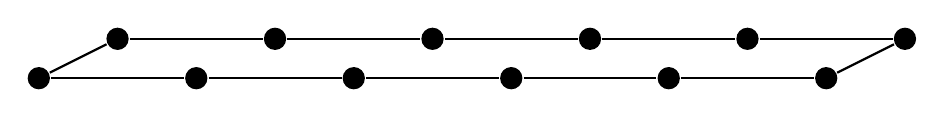
\begin{tikzpicture}[thick,inner sep=0.1cm]
	\node [fill,circle] (node 151878444) at (0.000000,0.000000) {};
	\node [fill,circle] (node 158252396) at (2.000000,0.000000) {};
	\node [fill,circle] (node 158252428) at (4.000000,0.000000) {};
	\node [fill,circle] (node 158252460) at (6.000000,0.000000) {};
	\node [fill,circle] (node 158252556) at (8.000000,0.000000) {};
	\node [fill,circle] (node 158252652) at (10.000000,0.000000) {};
	\node [fill,circle] (node 158252780) at (11.000000,0.500000) {};
	\node [fill,circle] (node 158252908) at (9.000000,0.500000) {};
	\node [fill,circle] (node 158253036) at (7.000000,0.500000) {};
	\node [fill,circle] (node 158384268) at (5.000000,0.500000) {};
	\node [fill,circle] (node 158384396) at (3.000000,0.500000) {};
	\node [fill,circle] (node 158384556) at (1.000000,0.500000) {};
	
	\draw (node 151878444) -- (node 158384556);
	\draw (node 151878444) -- (node 158252396);
	\draw (node 158252396) -- (node 158252428);
	\draw (node 158252428) -- (node 158252460);
	\draw (node 158252460) -- (node 158252556);
	\draw (node 158252556) -- (node 158252652);
	\draw (node 158252652) -- (node 158252780);
	\draw (node 158252780) -- (node 158252908);
	\draw (node 158252908) -- (node 158253036);
	\draw (node 158253036) -- (node 158384268);
	\draw (node 158384268) -- (node 158384396);
	\draw (node 158384396) -- (node 158384556);
\end{tikzpicture}

					\caption{Folded In Half}
					\label{fig:ringFolded}
				\end{subfigure}
				
				\vspace{2ex}
				
				\begin{subfigure}[b]{\textwidth}
					\center
					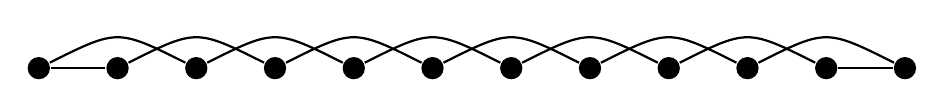
\begin{tikzpicture}[thick,inner sep=0.1cm]
	\node [fill,circle] (node 155478860) at (0.000000,0.000000) {};
	\node [fill,circle] (node 161861004) at (2.000000,0.000000) {};
	\node [fill,circle] (node 161861036) at (4.000000,0.000000) {};
	\node [fill,circle] (node 161861068) at (6.000000,0.000000) {};
	\node [fill,circle] (node 161861164) at (8.000000,0.000000) {};
	\node [fill,circle] (node 161861260) at (10.000000,0.000000) {};
	\node [fill,circle] (node 161861388) at (11.000000,0.000000) {};
	\node [fill,circle] (node 161861516) at (9.000000,0.000000) {};
	\node [fill,circle] (node 161988652) at (7.000000,0.000000) {};
	\node [fill,circle] (node 161988780) at (5.000000,0.000000) {};
	\node [fill,circle] (node 161988908) at (3.000000,0.000000) {};
	\node [fill,circle] (node 161989068) at (1.000000,0.000000) {};
	
	\draw (node 155478860) -- (node 161989068);
	\draw (node 155478860)
							         .. controls +(1.000000,0.500000)
							                 and +(-1.000000,0.500000)
							         .. (node 161861004);
	\draw (node 161861004)
							         .. controls +(1.000000,0.500000)
							                 and +(-1.000000,0.500000)
							         .. (node 161861036);
	\draw (node 161861036)
							         .. controls +(1.000000,0.500000)
							                 and +(-1.000000,0.500000)
							         .. (node 161861068);
	\draw (node 161861068)
							         .. controls +(1.000000,0.500000)
							                 and +(-1.000000,0.500000)
							         .. (node 161861164);
	\draw (node 161861164)
							         .. controls +(1.000000,0.500000)
							                 and +(-1.000000,0.500000)
							         .. (node 161861260);
	\draw (node 161861260) -- (node 161861388);
	\draw (node 161861388)
							         .. controls +(-1.000000,0.500000)
							                 and +(1.000000,0.500000)
							         .. (node 161861516);
	\draw (node 161861516)
							         .. controls +(-1.000000,0.500000)
							                 and +(1.000000,0.500000)
							         .. (node 161988652);
	\draw (node 161988652)
							         .. controls +(-1.000000,0.500000)
							                 and +(1.000000,0.500000)
							         .. (node 161988780);
	\draw (node 161988780)
							         .. controls +(-1.000000,0.500000)
							                 and +(1.000000,0.500000)
							         .. (node 161988908);
	\draw (node 161988908)
							         .. controls +(-1.000000,0.500000)
							                 and +(1.000000,0.500000)
							         .. (node 161989068);
\end{tikzpicture}

					\caption{Interleaved}
					\label{fig:ringInterleaved}
				\end{subfigure}
				
				\caption[Folding a ring network to reduce the maximum wire length]{The
				process of folding a ring network to reduce the maximum wire length}
				\label{fig:folding}
			\end{figure}
			
			This process is generalised to SpiNNaker's boards as shown in Figure
			\ref{fig:boardsFolded}.
			
			\begin{figure}
				\center
				\begin{subfigure}[b]{\textwidth}
					\center
					\input{|"python figures/boardsFoldedShift.py"}
					\caption{Shift left boards to the right to form a rectangle.}
					\label{fig:boardsFoldedShift}
				\end{subfigure}
				
				\vspace{2ex}
				
				\begin{subfigure}[b]{\textwidth}
					\center
					\input{|"python figures/boardsFoldedSpaced.py"}
					\caption{Fold along the gaps in this figure. Wires omitted for
					clarity.}
					\label{fig:boardsFoldedSpaced}
				\end{subfigure}
				
				\vspace{2ex}
				
				\begin{subfigure}[b]{\textwidth}
					\center
					\input{|"python figures/boardsFoldedInterleaved.py"}
					\caption{The (more complex) wiring after folding. Redrawn with squares
					as hexagons don't visually fit together after folding and
					interleaving.}
					\label{fig:boardsFoldedInterleaved}
				\end{subfigure}
				
				\caption[Folding SpiNNaker]{The process of folding SpiNNaker. Coloured
				lines represent wires travelling {\color{red}North/South},
				{\color{green}North-East/South-West} and {\color{blue}East/West}}
				\label{fig:boardsFolded}
			\end{figure}
			
			The first step (Figure \ref{fig:boardsFoldedShift}) transforms the
			rhombus-like arrangement of boards into a rectangle which is more easily
			folded.
			
			In the next step, the design is folded into four parts on the X-axis and
			into two on the Y-axis (Figure \ref{fig:boardsFoldedSpaced}). It is
			necessary to fold the X-axis into four as the long, diagonal wires don't
			cross the entire system on the X-axis and instead reach half way. Folding
			in two would not bring these points any closer\footnote{For example, the
			wire travelling from the bottom left board to the top-middle board after
			folding in two would now have to cross from one end of the system to the
			other -- an even longer distance than it had to before.} while folding
			into four brings them next to each other. As a result, the maximum wire
			length is reduced.
			
			The final step in the process is to map the boards into their real-world
			physical positions. The largest SpiNNaker system will be installed into a
			series of cabinets, each containing a number of racks (shelves) into which
			the boards are slotted and wired up. Figure \ref{fig:spinnaker106} shows a
			possible rack placement scheme for the largest planned SpiNNaker system.
			
			\begin{figure}
				\center
				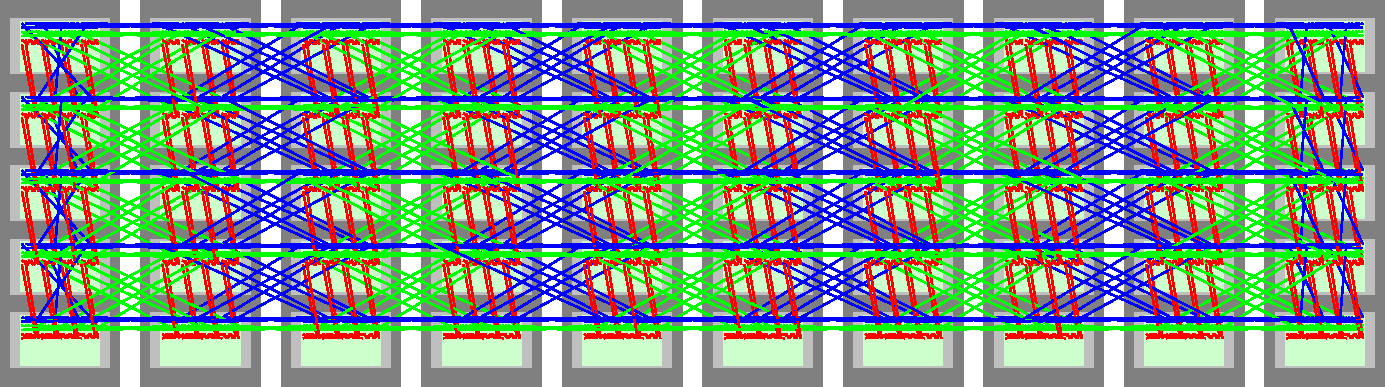
\includegraphics[width=\textwidth]{figures/spinnaker106}
				\caption[The largest SpiNNaker machine mapped into cabinets and
				racks]{The largest SpiNNaker machine with 1,200 boards ($20\times20$
				threeboards) and 1,036,800 cores mapped into 10 cabinets of 5 racks
				each.  Coloured lines represent wires connecting
				{\color{red}North/South}, {\color{green}North-East/South-West} and
				{\color{blue}East/West} links}
				\label{fig:spinnaker106}
			\end{figure}
			
			Even though the system is physically several meters long, the longest wire
			will only be around one meter in length which is within the tolerances of
			the high-speed link technology. This placement scheme, therefore, meets the
			wire-length requirement.
			
		\subsection{Wiring Complexity}
			
			The final concern for the wiring is that it should not be too complex to
			be completed by hand. The large-scale SpiNNaker machine will contain 3,600
			wires and so it is clearly not practical to have to look up each
			individual connection before wiring it up. Though it is clear that the
			folded arrangement is substantially less regular than the original layout,
			some regularity remains.
			
			For example, it is easy to see that wires making connections for a
			particular direction (shown by the different colours in Figure
			\ref{fig:spinnaker106} show a moderate degree of regularity. In addition,
			the wiring for the North/South direction (shown in red) remains entirely
			within a cabinet.
			
			By splitting up the wiring tasks by the logical direction (and thus by the
			connector on the board) it is clear that a large amount of regularity
			exists in each group of wires (see the different colours in Figure
			\ref{fig:spinnaker106}). If the task is further split depending on whether
			the wires stay with in a rack or cabinet, batches of identical racks and
			cabinets can be wired up independently before being linked together later.
			For example, the wires connecting North to South (shown in red) remain
			entirely within a cabinet meaning all North/South wiring can be completed
			independently for each cabinet.
			
			Based on the above partitioning scheme, the connections for all 3,600
			wires can be described using only 53 instructions. This satisfies the
			final constraint on wiring complexity.
		
		\subsection{`SpiNNer' Wiring Guide Generator}
			
			As part of this work SpiNNaker, a wiring modelling library and wiring
			guide generator, was produced to assist in the construction of SpiNNaker
			systems consisting of multiple boards. These tools helped avoid the error
			prone process of manually visualising the various transformations.
			
			The modelling library allows transformations, such as folding, to be
			easily applied to a network of boards. From the transformed network,
			various measurements such as the maximum physical wire length can then be
			directly determined. Using this library the largest SpiNNaker machine can
			be described in 10 lines of code\footnote{This number includes only the
			`functional' lines of code does not include `boilerplate' code for
			importing libraries nor definitions of the physical dimensions of cabinets
			and racks.}.
			
			The wiring guide generator produces illustrated\footnote{Many of the
			figures in this section were adapted from wiring guides generated by
			SpiNNer.} documents using \LaTeX{} which describe the wiring for
			arbitrarily sized machines. Metrics such as the distribution of wire
			lengths are included along with instructions for wiring the system up. At
			the time of writing, the largest prototype system constructed, a single
			threeboard, has been successfully wired up in a manner consistent with the
			generated wiring guide.
		
		\subsection{Further Work}
			
			% Simplify instructions, alternative wirings.
			
			The wiring guide generator is currently only capable of producing
			exhaustive wiring descriptions with one instruction for each of the 3,200
			wires. The foundations for extracting regularity currently exist in
			experimental form and must eventually be integrated into the wiring guide
			generator.
			
			In addition, further work may be carried out to propose alternative wiring
			schemes. The current scheme, a huge number of wires cross between
			different cabinets. As a result a significant amount of the wiring cannot
			be done in isolated batches. An alternative scheme may be able to reduce
			this number and further simplify the task of wiring.
	
	\section{Small-World Super Computers}
		
		In the same way that random search is generic (no free lunch), I tried
		adding random wires. This is backed up by Watts and Strogatz's small-world
		network producing algorithm. Built a model. Took into account wiring using
		techniques in Wiring-Up Super Computers.
		
		\subsection{Results}
			
			Even with wire-length limits in place, when folded the effect is still
			noticeable.
		
		\subsection{Further Work}
			
			Must try this with SpiNNaker topology and racks (maybe even better). Would
			like to formalise the result into a formula.
	
	\section{Place and Route}
		
		Tests written for the Place and Route system for SpiNNaker-103. Gained some
		experience with the task. 
		
		\subsection{Potential Improvements}
			
			The algorithms used for placement and routing are naive: generally greedy
			algorithms.



